\documentclass{article}

\usepackage[version=3]{mhchem} % Package for chemical equation typesetting
\usepackage{siunitx} % Provides the \SI{}{} and \si{} command for typesetting SI units
\usepackage{graphicx} % Required for the inclusion of images
\usepackage{natbib} % Required to change bibliography style to APA
\usepackage{amsmath} % Required for some math elements 
\usepackage{graphicx}
\usepackage{comment}
\usepackage{amsmath}
\usepackage{amsfonts}
\usepackage{amssymb}
\usepackage[margin=1in]{geometry}
\usepackage{textcomp}






\title{Study of Diode Rectifier Circuits \\ EEE-2302} % Title

\author{Mohammad \textsc{Zakaria}} % Author name

\date{\today} % Date for the report

\begin{document}
	
	\maketitle % Insert the title, author and date
	
	\begin{center}
		\begin{tabular}{l r}
			Date Performed: & January 31, 2021 \\ % Date the experiment was performed
			% Partners: & James Smith \\ % Partner names
			% & Mary Smith \\
			Instructor: & Lokman Hossain % Instructor/supervisor
		\end{tabular}
	\end{center}
	
	
	\section{Objective:}
	
	To understand principle of diode in converting ac into dc and to study different diode rectifier circuits.
	
	
	\section{Objective:}
	To understand principle of diode in converting ac into dc and to study different diode rectifier circuits.
	
	
	\section{Theory:}
	The diode rectifier converts the input sinusoidal voltage $V_s$ to a uni-polar output $V_o$. There are
	two types of rectifier circuits: (i) Half-wave rectifier and (ii) Full-wave rectifier.
	
%	\subsection{PIV (Peak Inverse Voltage)}
	\begin{description}
		\item[PIV]  is the peak inverse voltage that appears across the diode when it is reverse-biased. For half wave
		rectifier $PIV = V_m$
	\end{description}
	
%	\subsection{Ripple Factor:}
		\begin{description}
			\item[Ripple factor:]  A rectifier converts alternating currents into a unidirectional current, periodically fluctuating components
			still remaining in the output wave. A measure of the fluctuating component is given by the ripple factor r,
			which is defined as
			r = RMS value of alternating components of wave/Average value of wave
			For a half-wave rectifier, r = 1.21 and for a full wave rectifier r = 0.482
		\end{description}

		\begin{description}
			\item[Filter:] The rectifier with a filter is shown in Fig 1. When capacitor charges to Vp(12V p-p), input voltage decreases
			immediately but capacitor will not charge its voltage instantaneously. As a result diode will be reverse
			biased and stop conducting. The stored charges on the capacitor will be released through R.
		\end{description}

	
	
	\section{Equipments:}
	\begin{tabular}{ll}
		Trainer board \\
		Multimeter \\
		Resistor \\
		Capacitor 1\textmu F,\ 47\textmu F, \ 220\textmu F, 1000\textmu F \\
		Diode \ & 4 pieces \\
	\end{tabular}
	
	
	
	
	\section{Circuit Diagram:}
	
	\begin{figure}[!htb]
		\begin{center}
			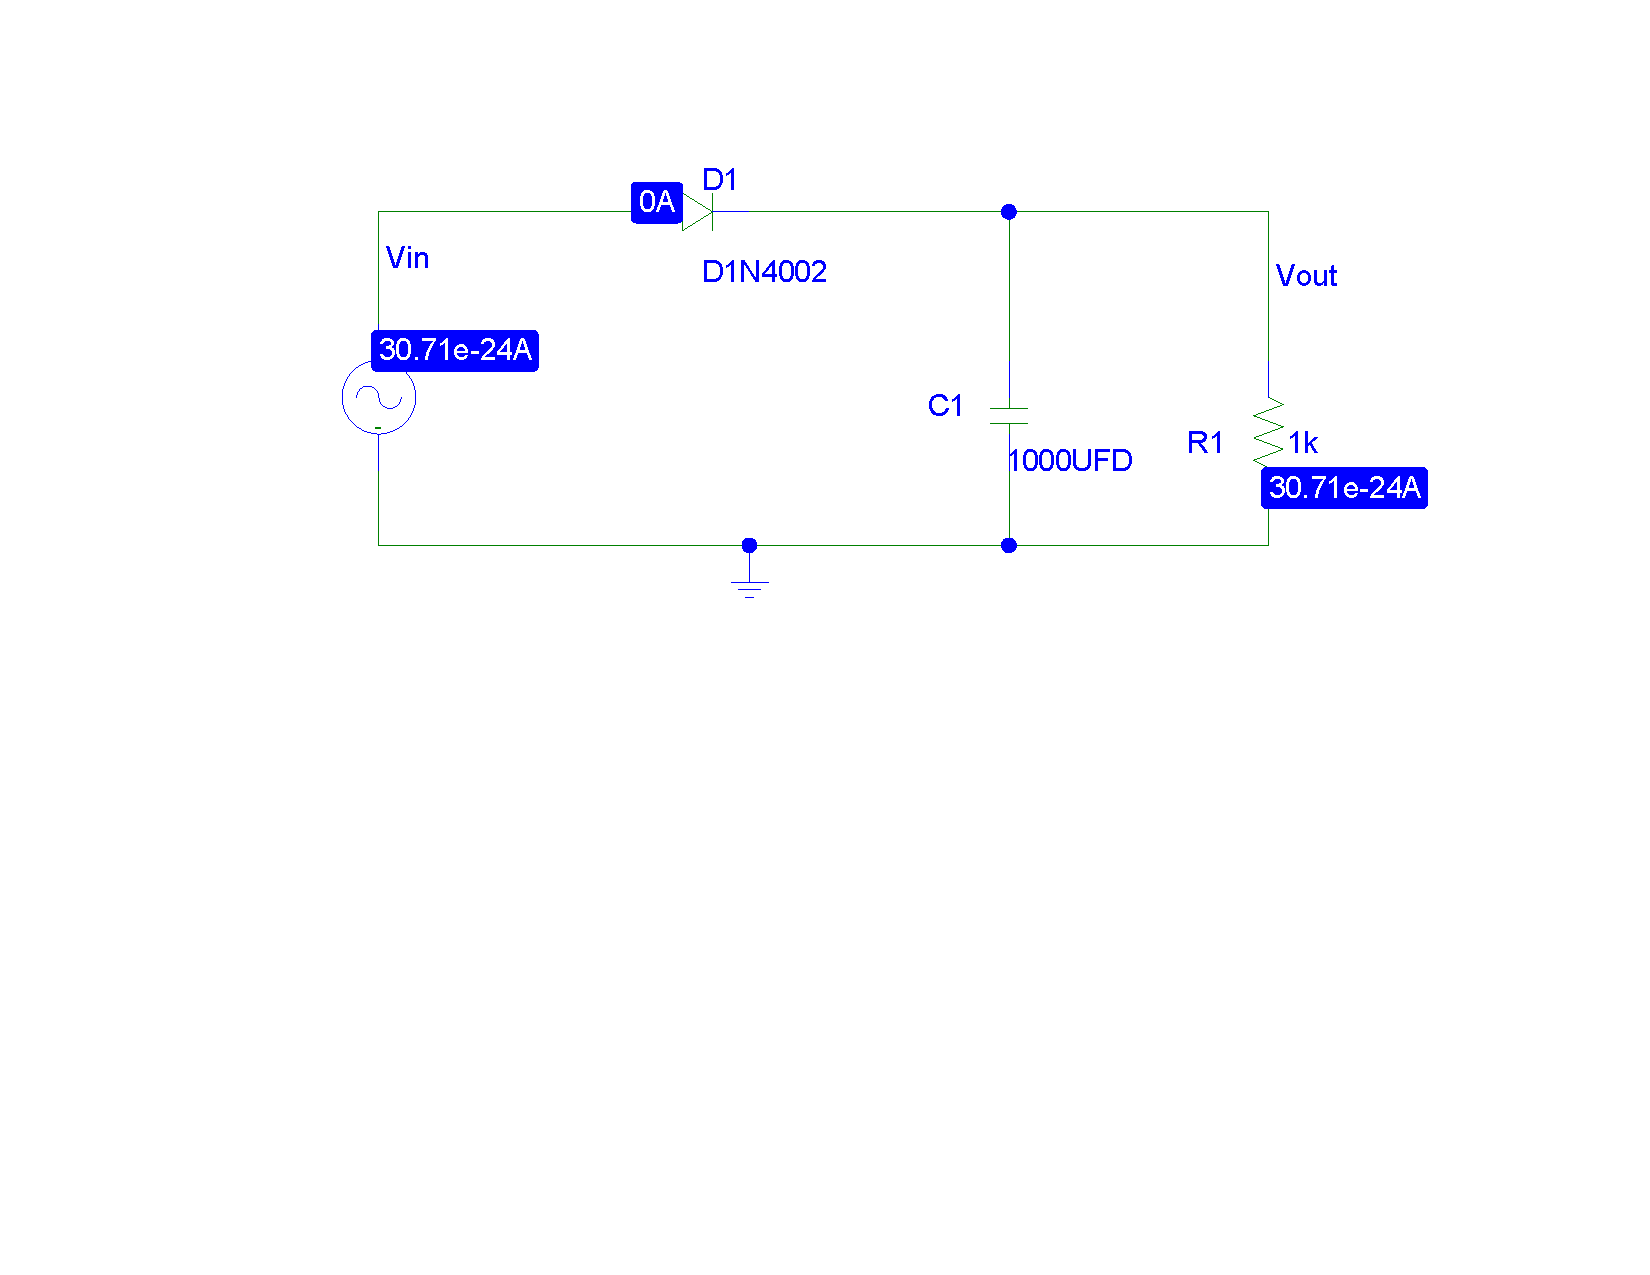
\includegraphics[width=0.65\textwidth]{ckt-diagram-halfwave.pdf} % Include the image placeholder.png
			\caption{Circuit diagram for half-wave rectifier.}
		\end{center}
	\label{fig:halfwave rectifier} 	The input and output of the rectifier are drawn in fig. 1. Diode conducts only when it is forward biased. For $V_s = V_m sin\omega t$, DC voltage of a half wave rectifier is $V_{DC} = (V_m -V_T) / \pi $ ; where $V_T \approxeq 0.7 $ \\
	
	\end{figure}



\begin{figure}[!htb]
	\centering
	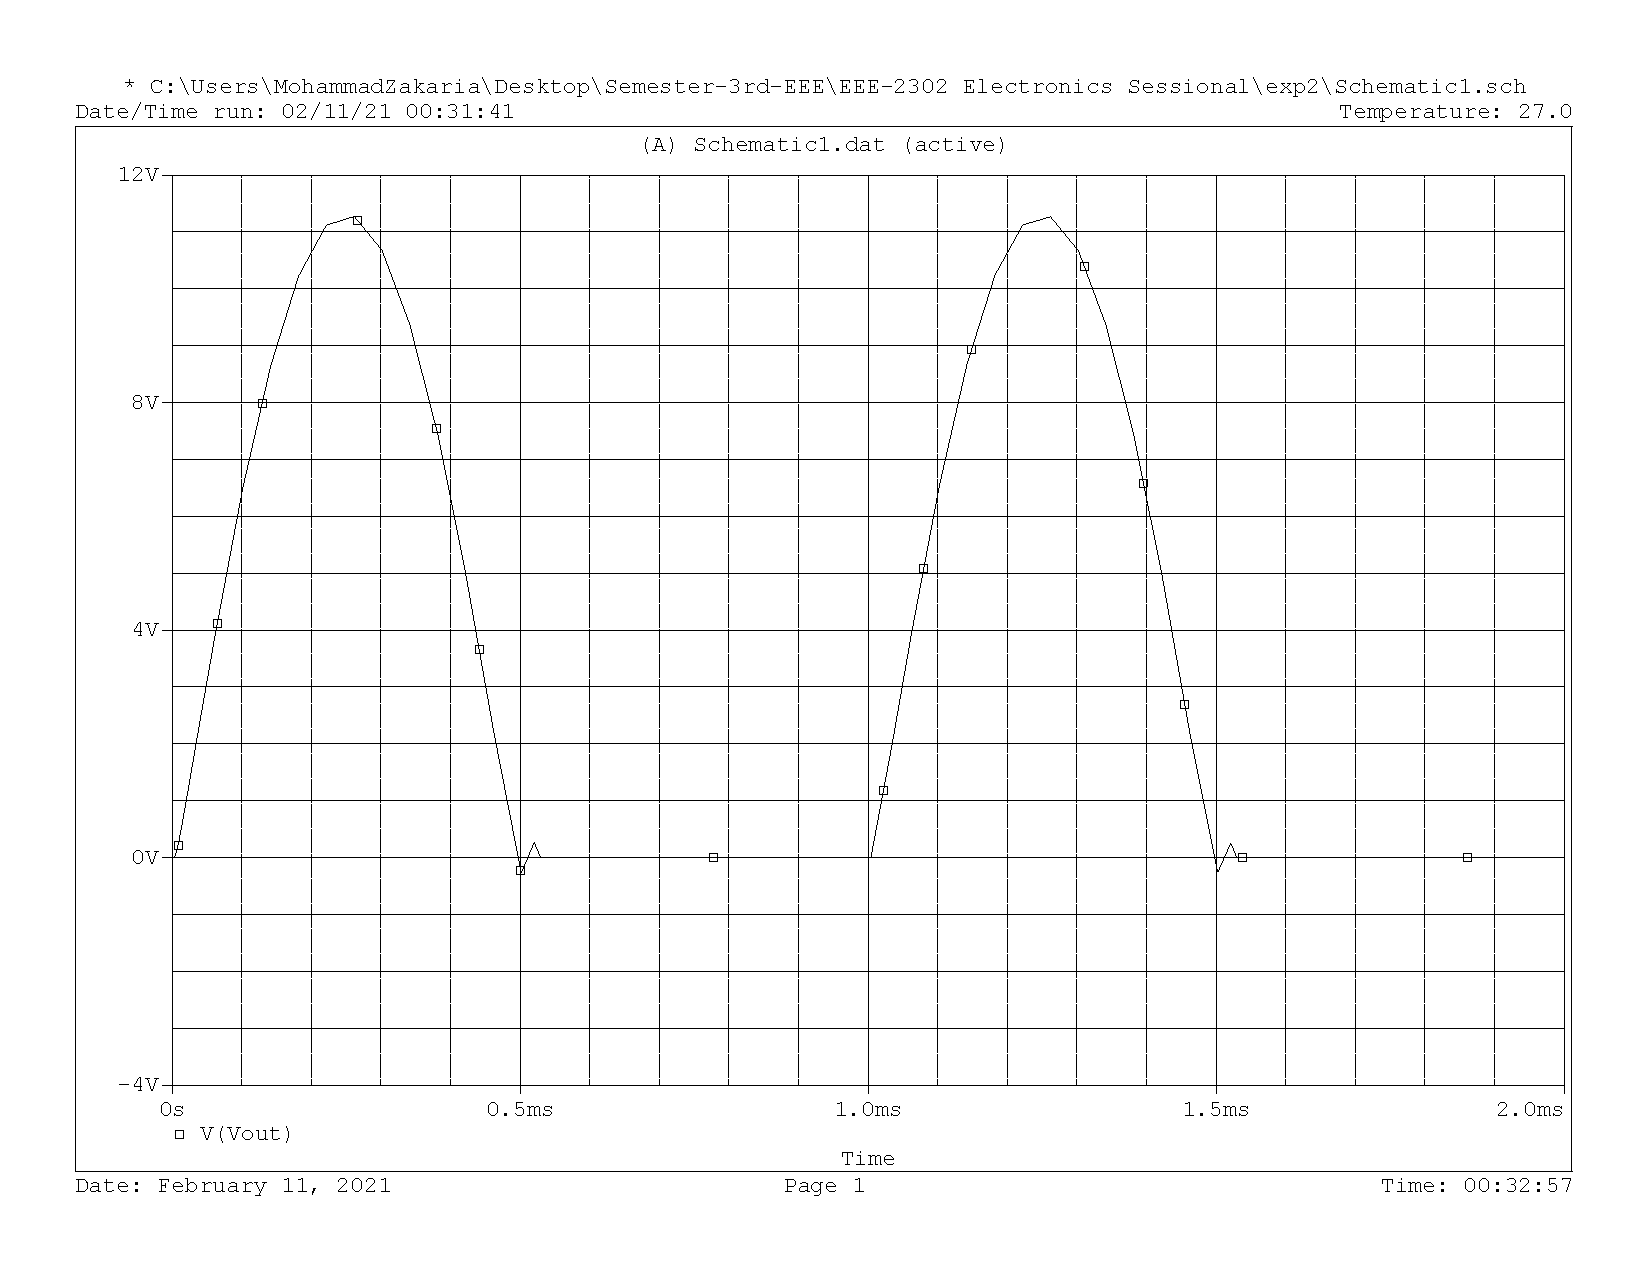
\includegraphics[width=0.7\linewidth]{Vout1}
	\caption{}
	\label{fig:vout1} Output voltage, when no capacitor is connected. Output is pulsating dc.
\end{figure}

\begin{figure}[!htb]
	\centering
	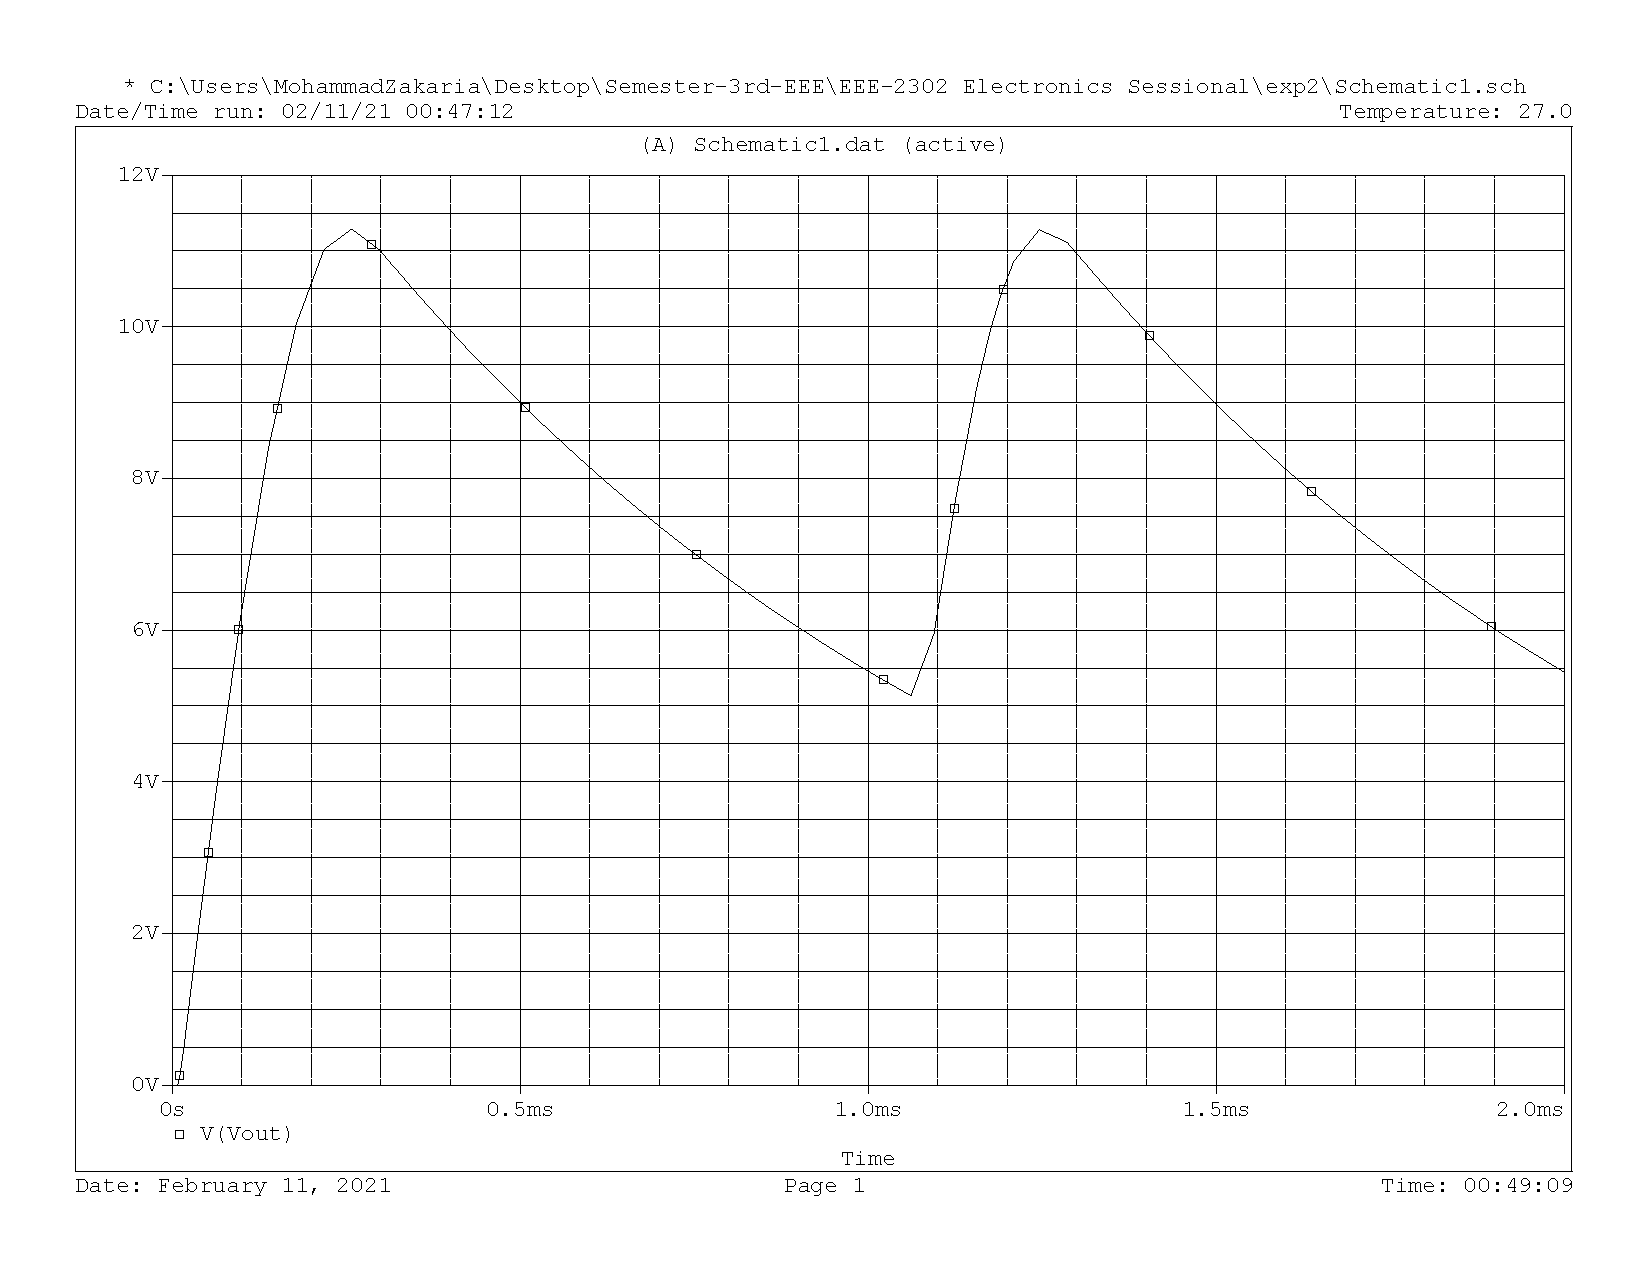
\includegraphics[width=0.7\linewidth]{Vout-for-1UFD-capacitor}
	\caption{}
	\label{fig:vout-for-1ufd-capacitor} Output voltage when 1\textmu F capacitor is connected in parallel with the load. Ripple is decreasing, still this is not pure dc.
\end{figure}
	
\begin{figure}[!htb]
	\centering
	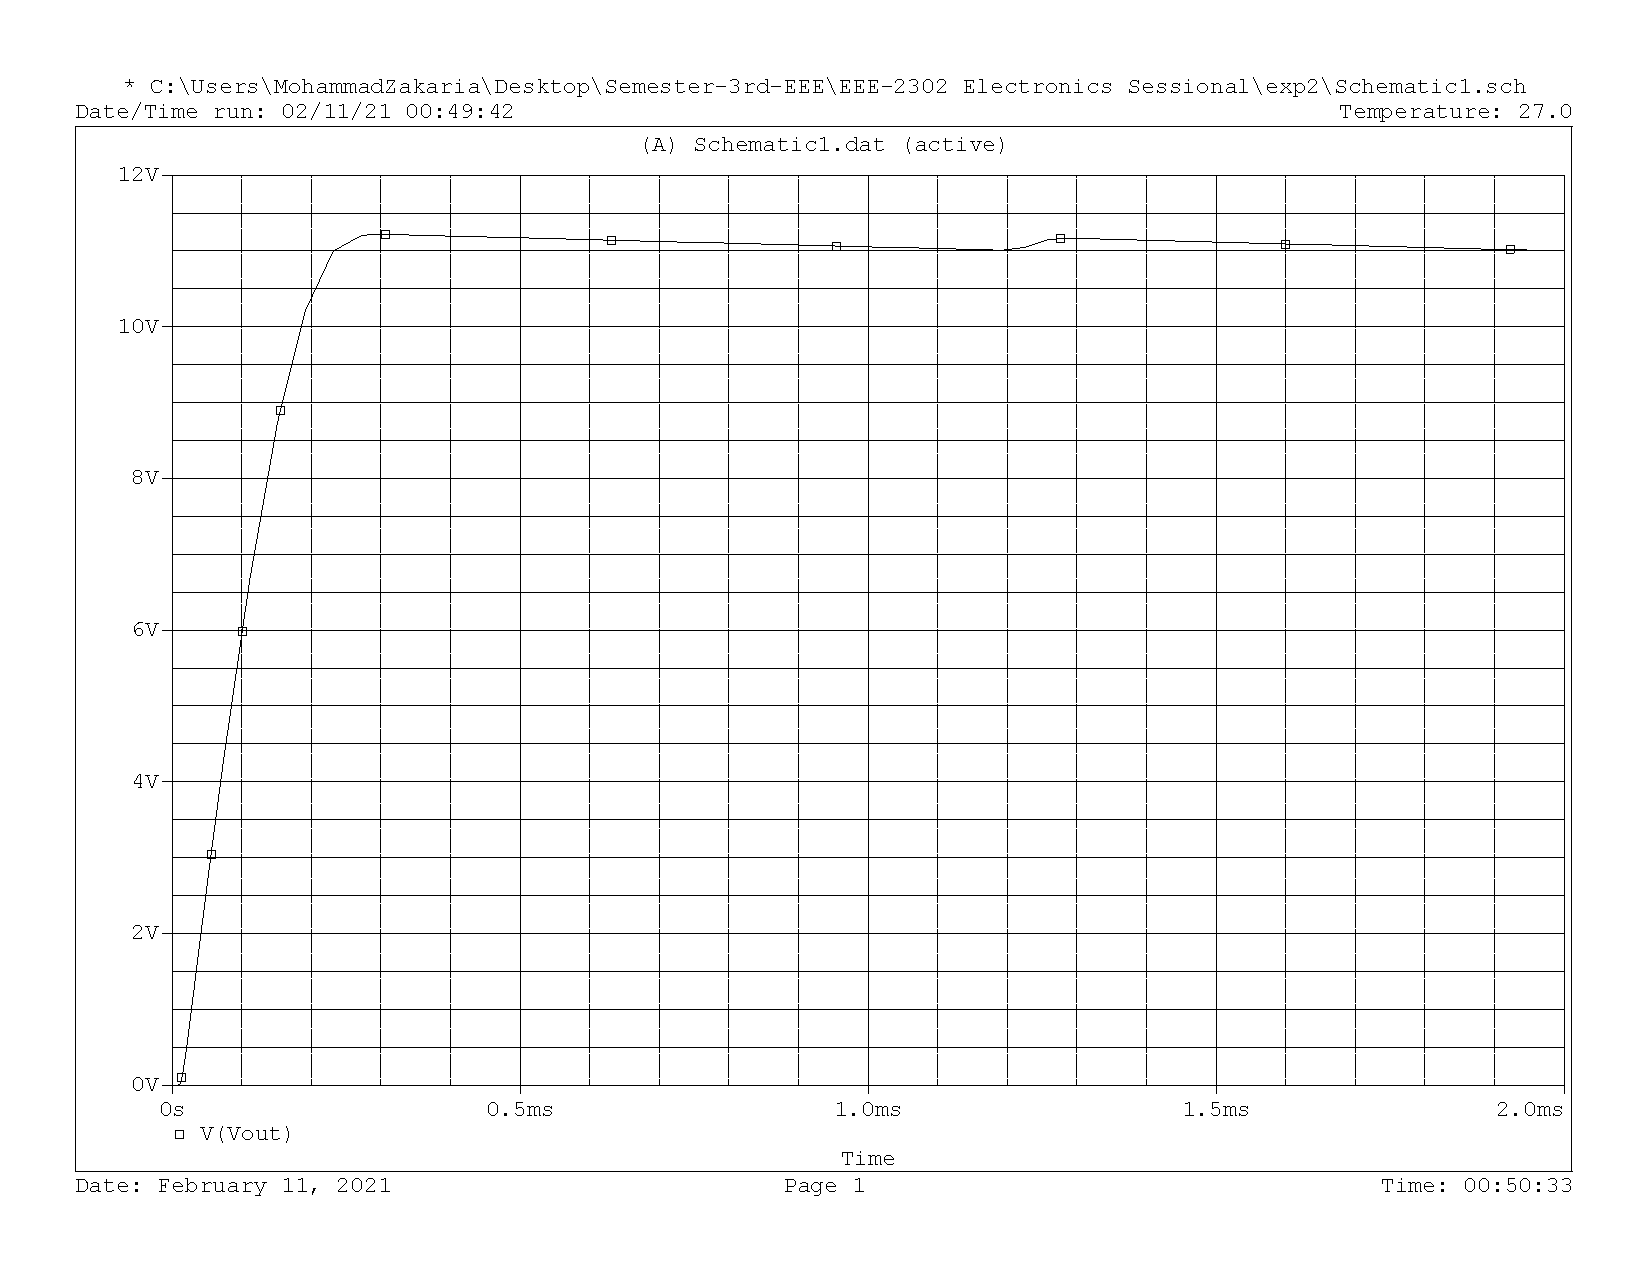
\includegraphics[width=0.7\linewidth]{Vout-for-47UFD}
	\caption{}
	\label{fig:vout-for-47ufd} This is almost nearer to pure dc.
\end{figure}

	\begin{figure}[!htb]
		\centering
		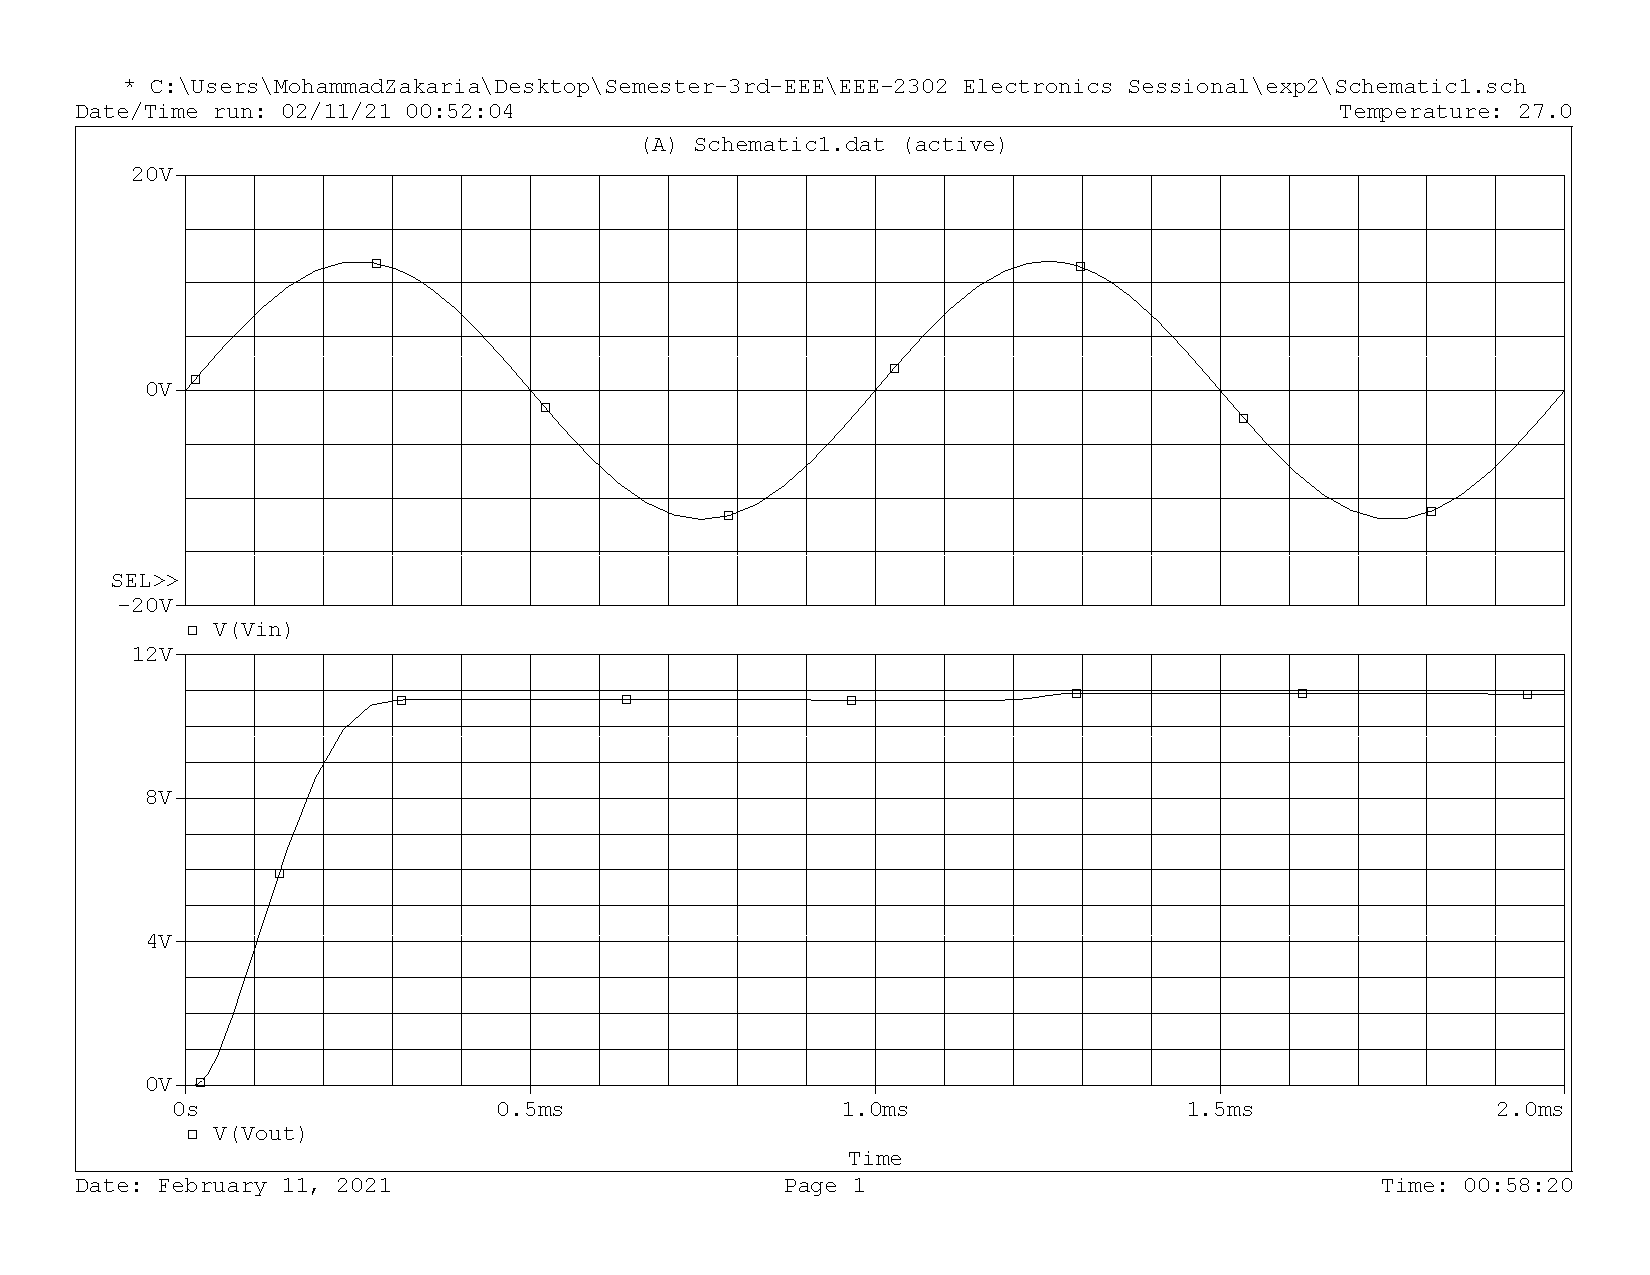
\includegraphics[width=0.7\linewidth]{Vout-and-Vin-for-halfwavefinal}
		\caption{}
		\label{fig:vout-and-vin-for-halfwavefinal} Input and output voltage curve for half-wave rectifier. Here we connected 220\textmu F capacitor. From the simulation graph the output seems to pure dc.
	\end{figure}

% Full wave bridge rectifier

	
	\begin{figure}[!htb]
		\begin{center}
			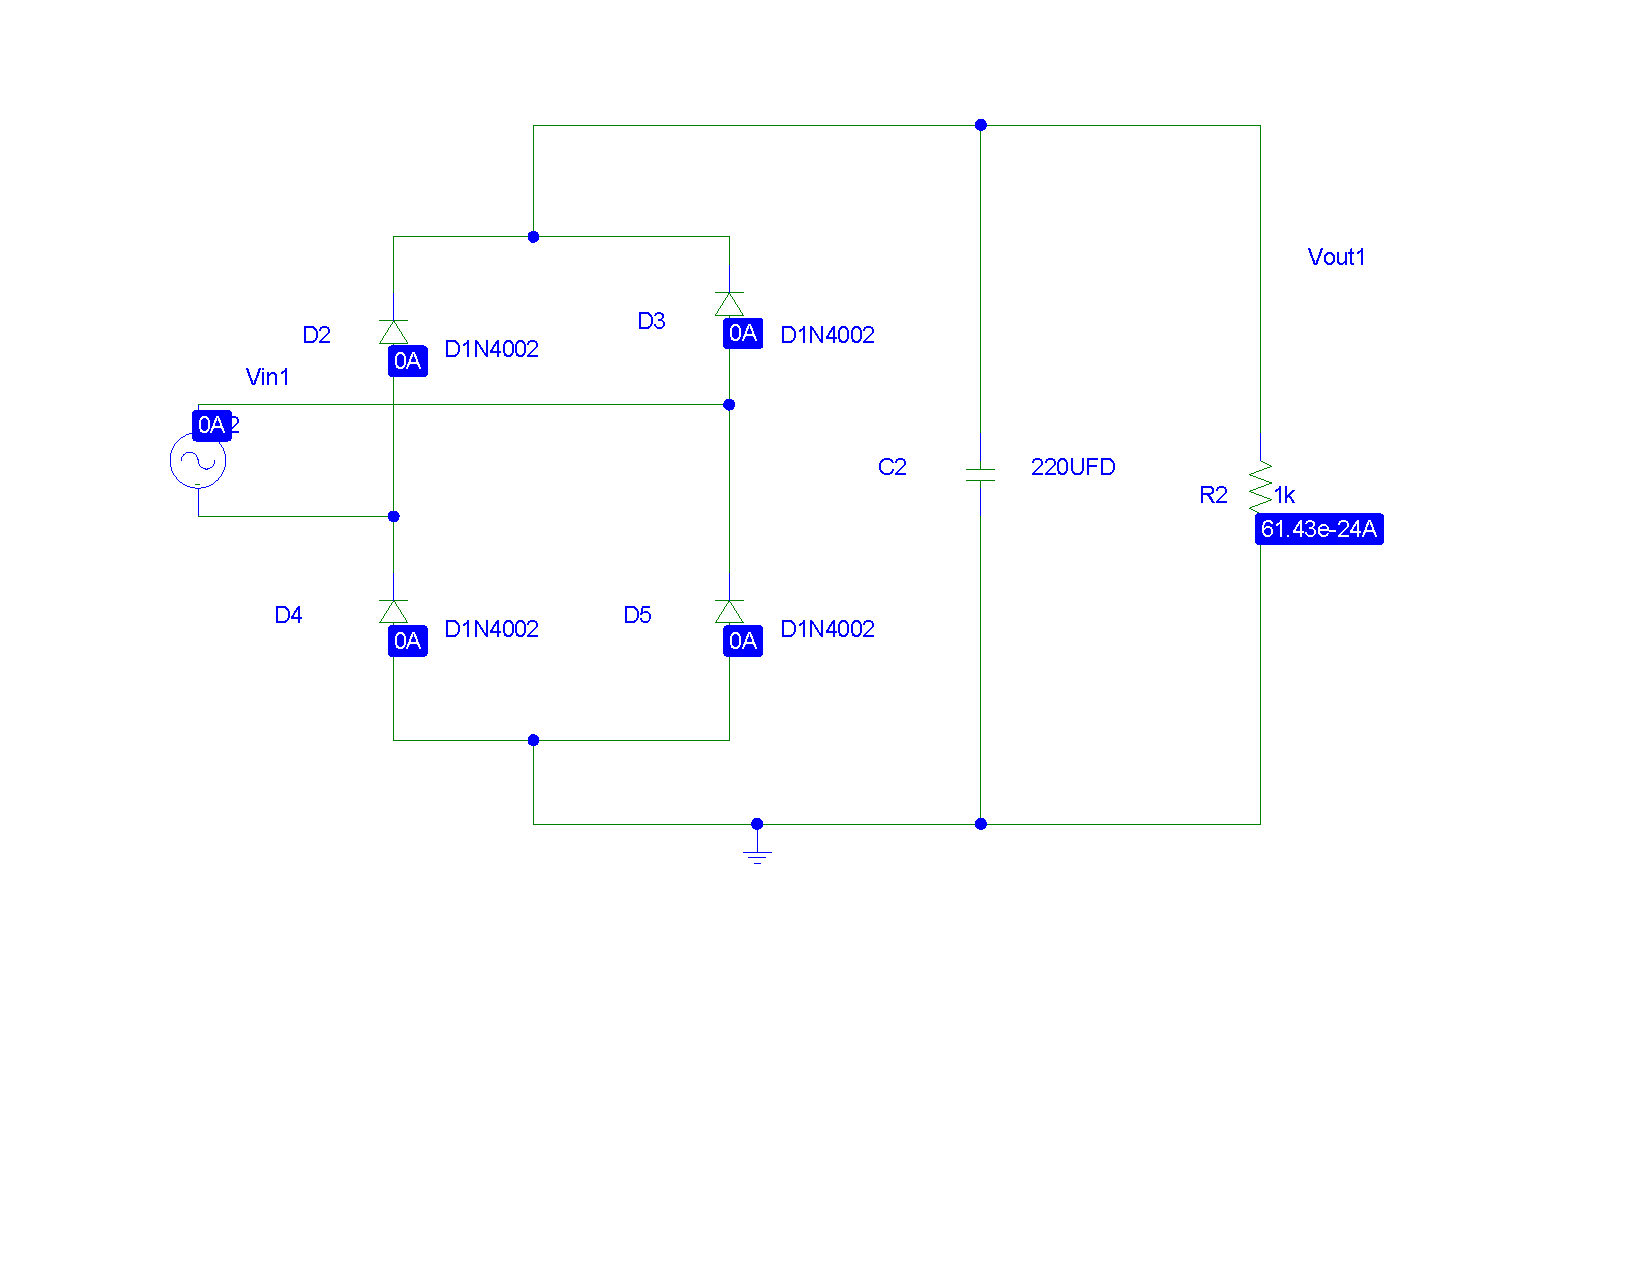
\includegraphics[width=0.65\textwidth]{ckt-diagram-fullwave.pdf} % Include the image placeholder.png
			\caption{Circuit diagram for bridge rectifier.}
		\end{center}
	\end{figure}	


	\begin{figure}[!htb]
		\centering
		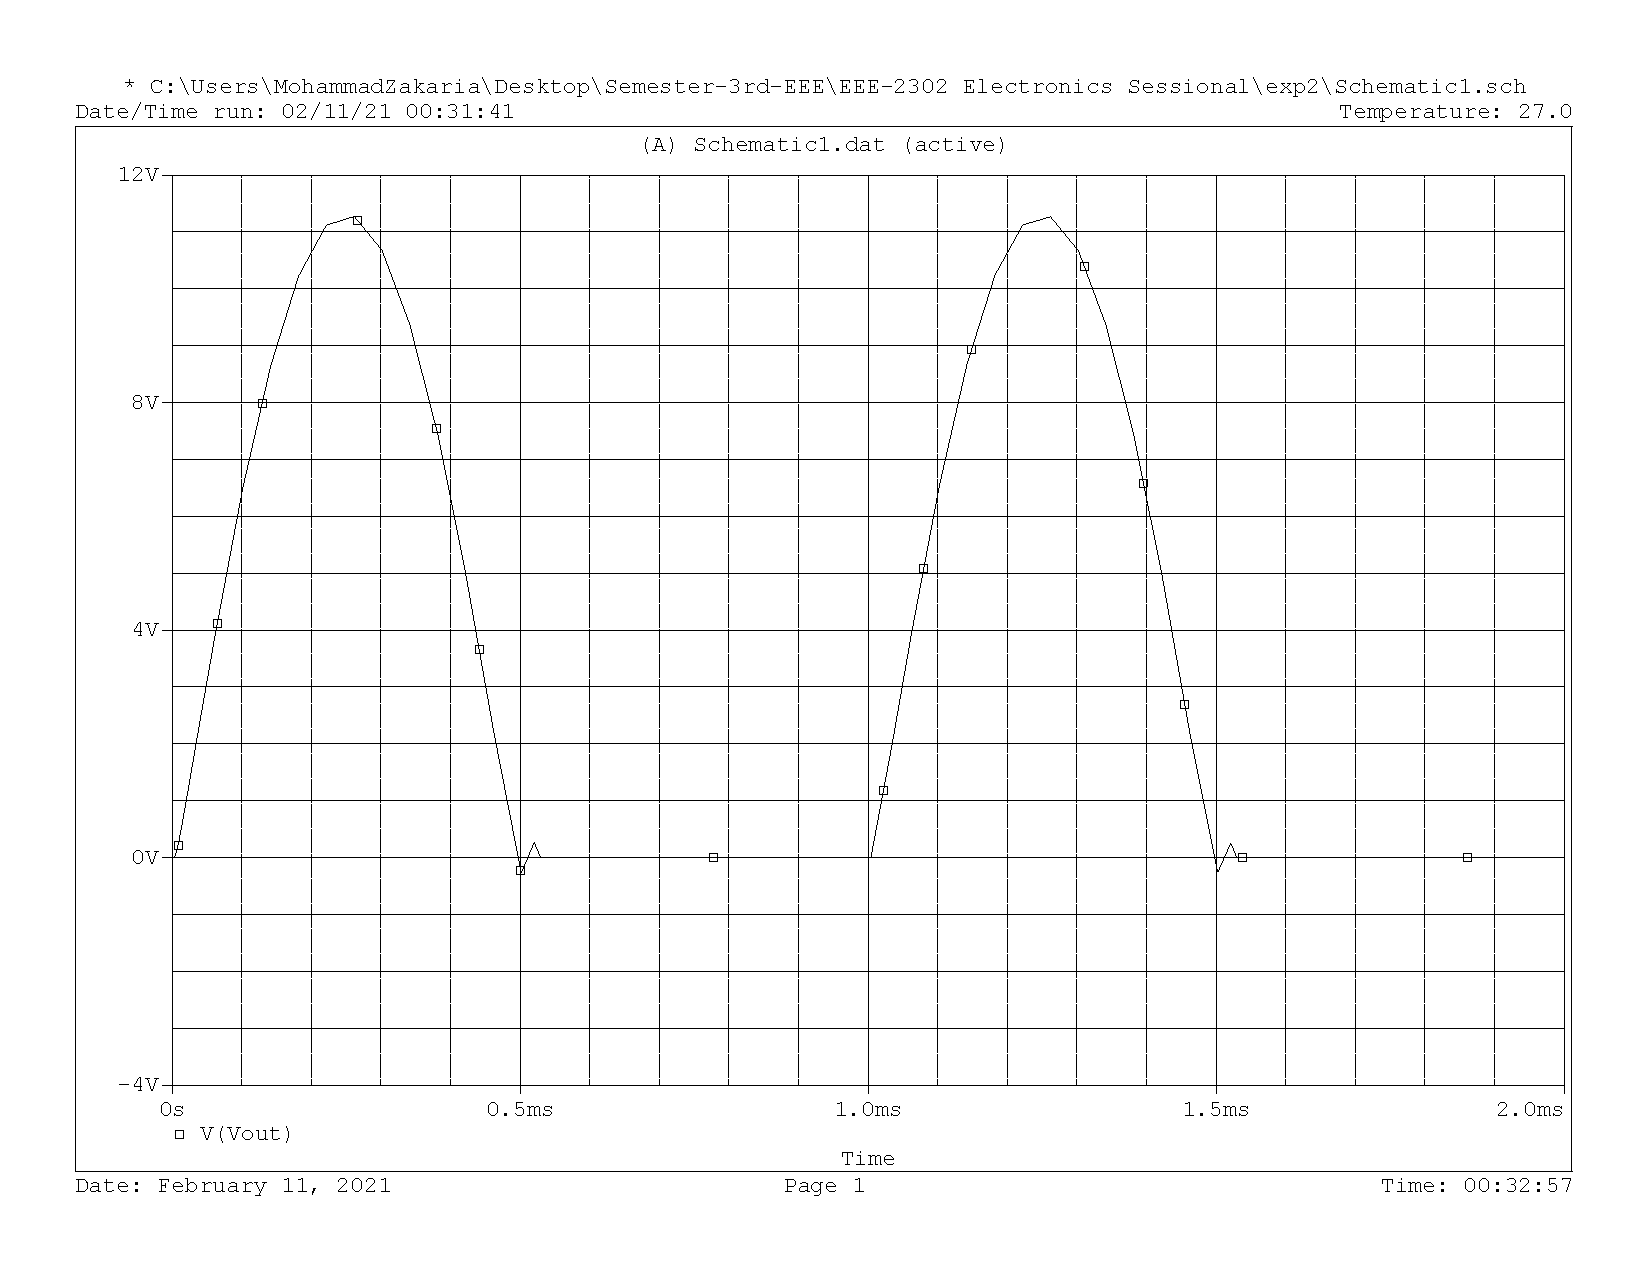
\includegraphics[width=0.7\linewidth]{Vout1}
		\caption{}
		\label{fig:vout1} Output voltage for full wave bridge rectifier when no capacitor is connected.
	\end{figure}
	
	
	\begin{figure}[!htb]
	\begin{center}
		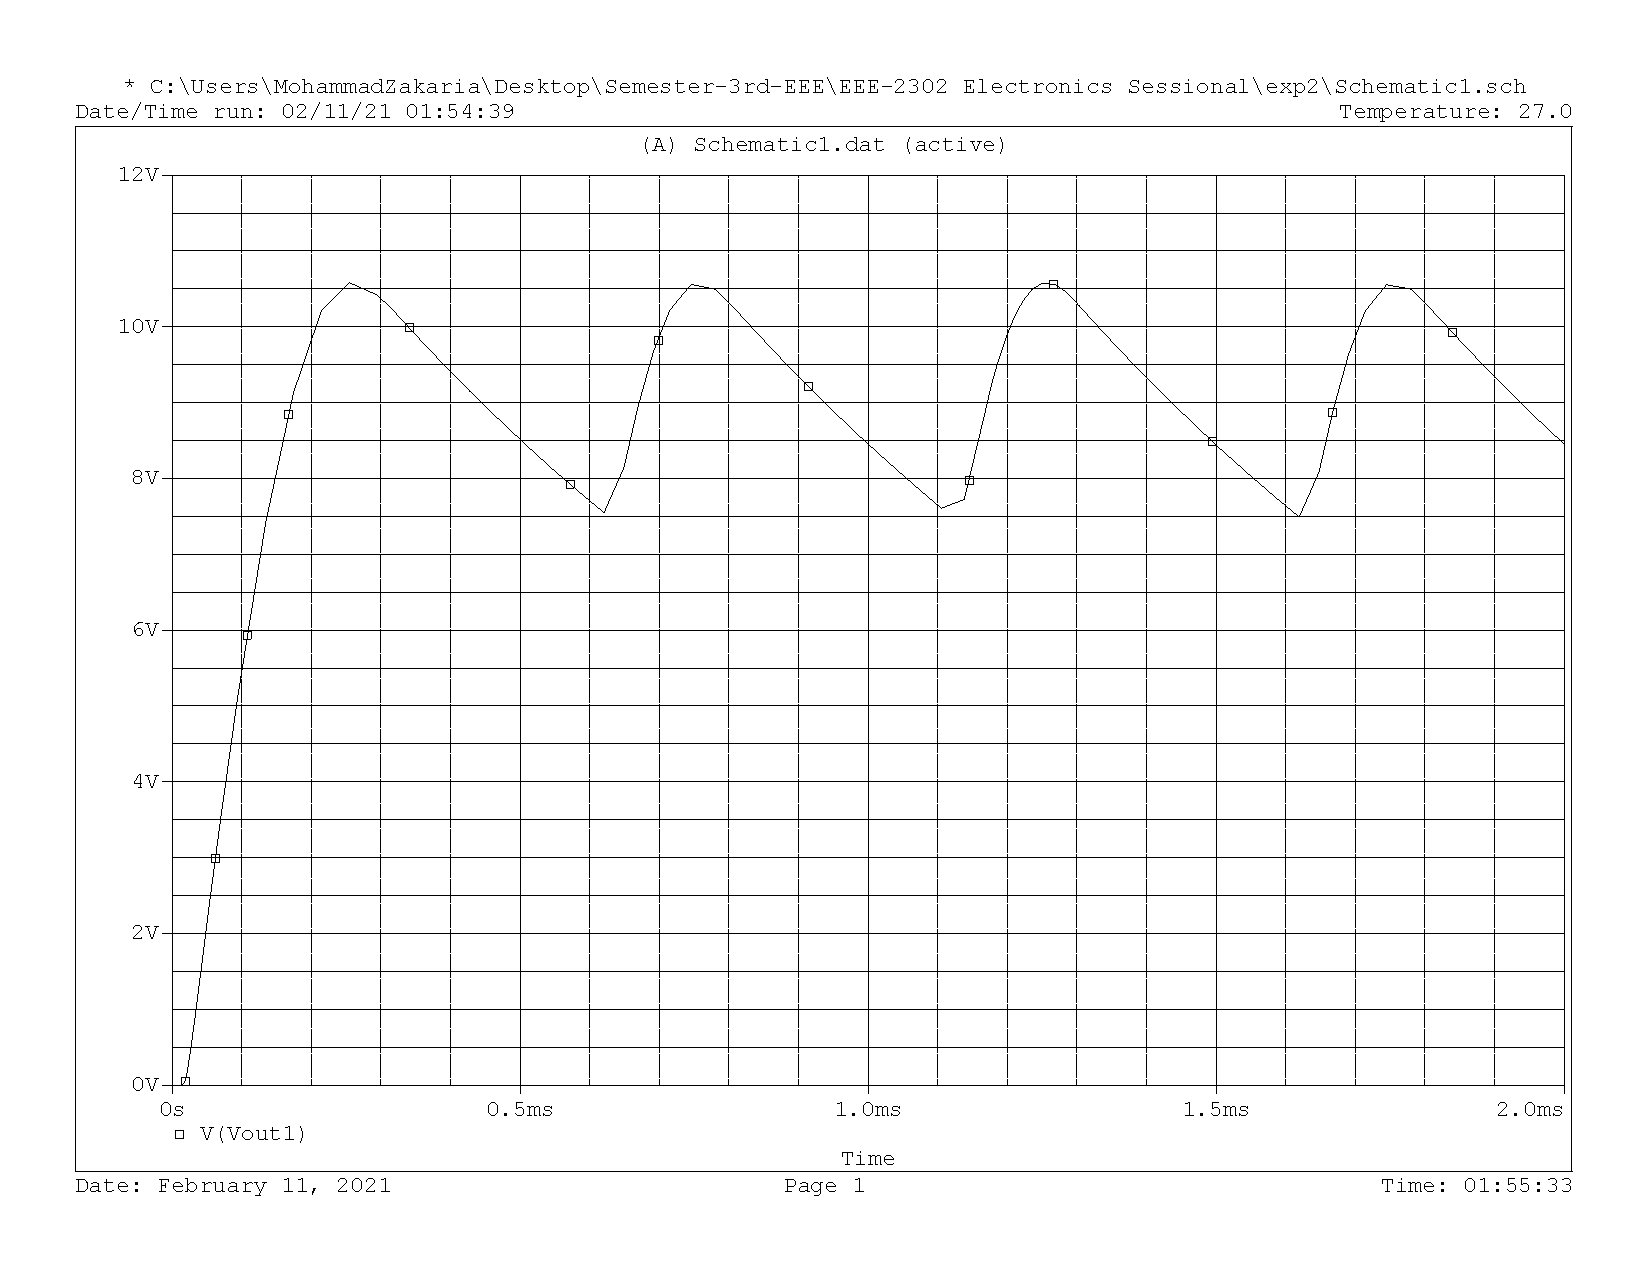
\includegraphics[width=0.65\textwidth]{Vout1-for-bride-fullwave-with-1ufd-capacitor.pdf} % Include the image placeholder.png
		\caption{} Output voltage curve, when 1 \textmu F capacitor is connected in parallel with the load.
	\end{center}
	\end{figure}



	\begin{figure}[!htb]
	\begin{center}
		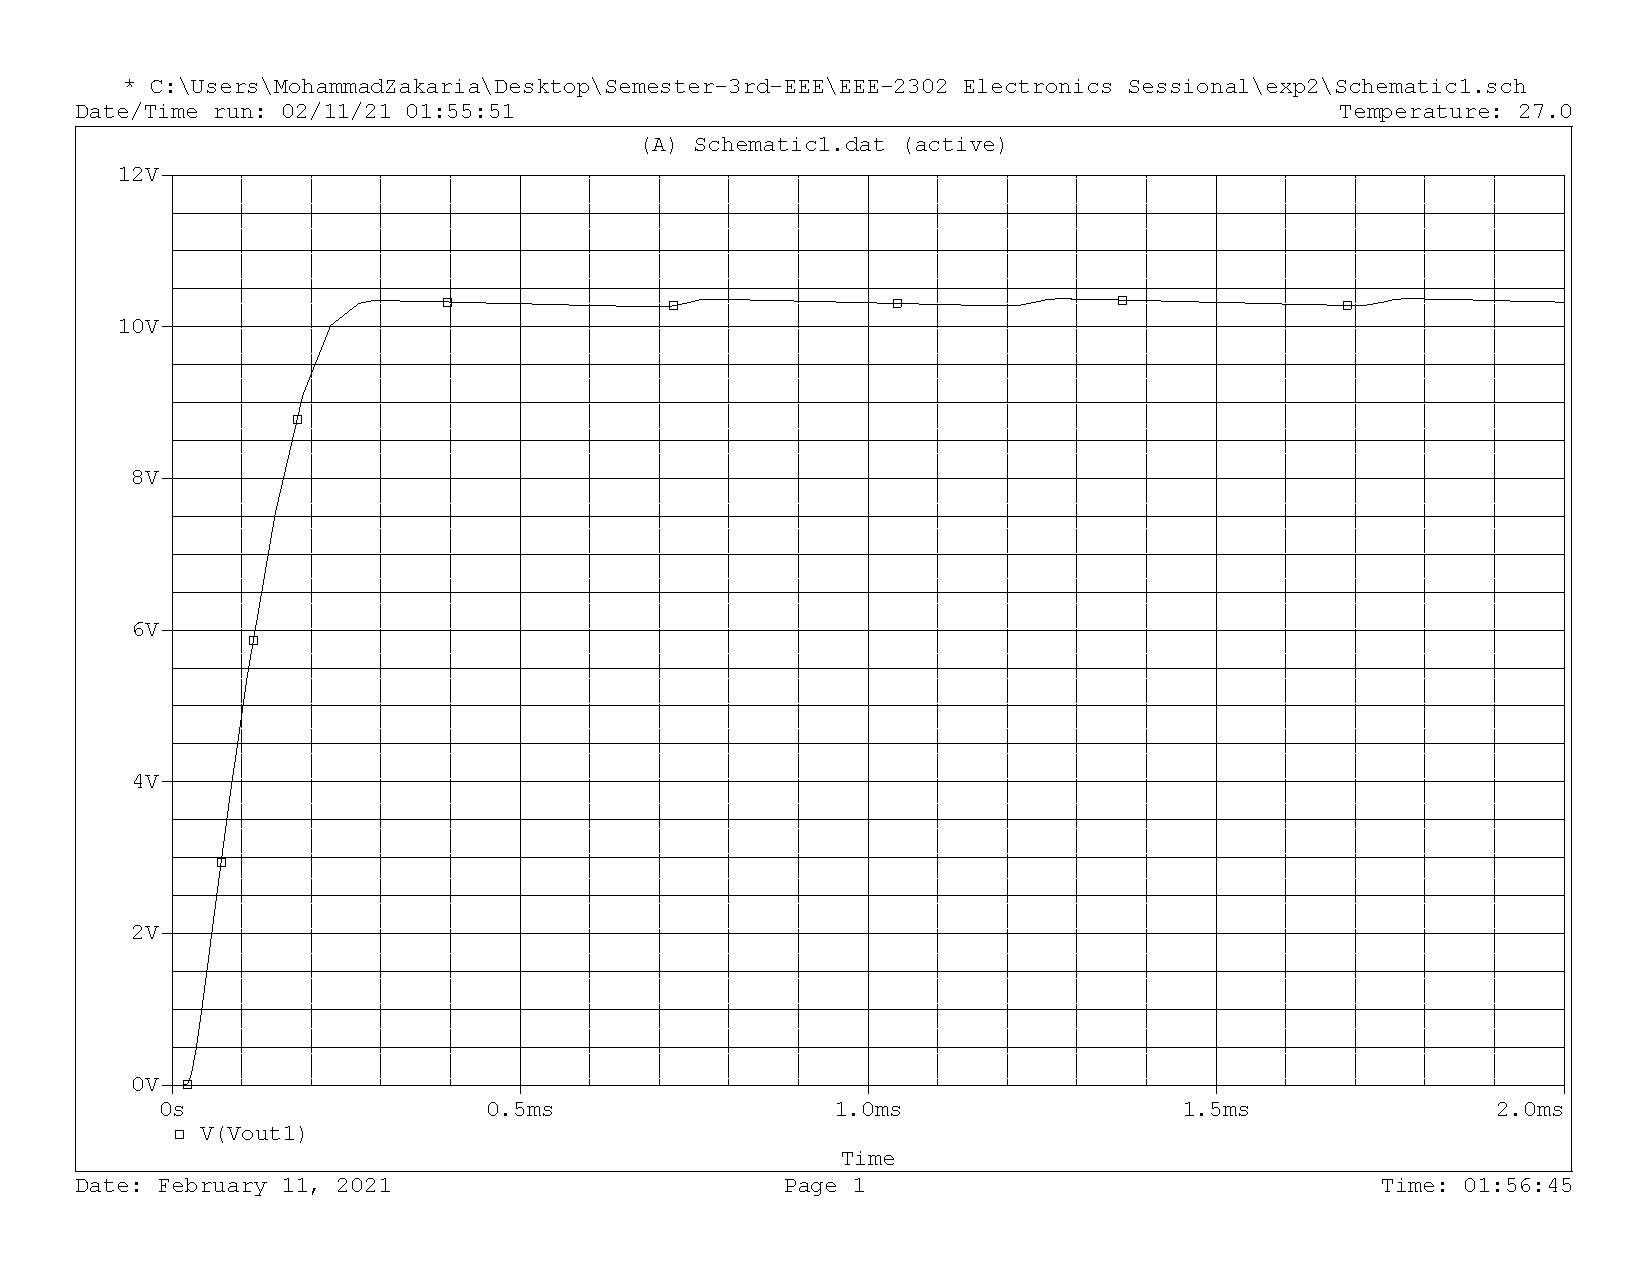
\includegraphics[width=0.65\textwidth]{Vout1-for-bride-fullwave-with-47ufd-capacitor.pdf} % Include the image placeholder.png
		\caption{} Output voltage curve, when 47 \textmu F capacitor is connected in parallel with the load.
	\end{center}
	\end{figure}
	
	
	\begin{figure}[!htb]
		\centering
		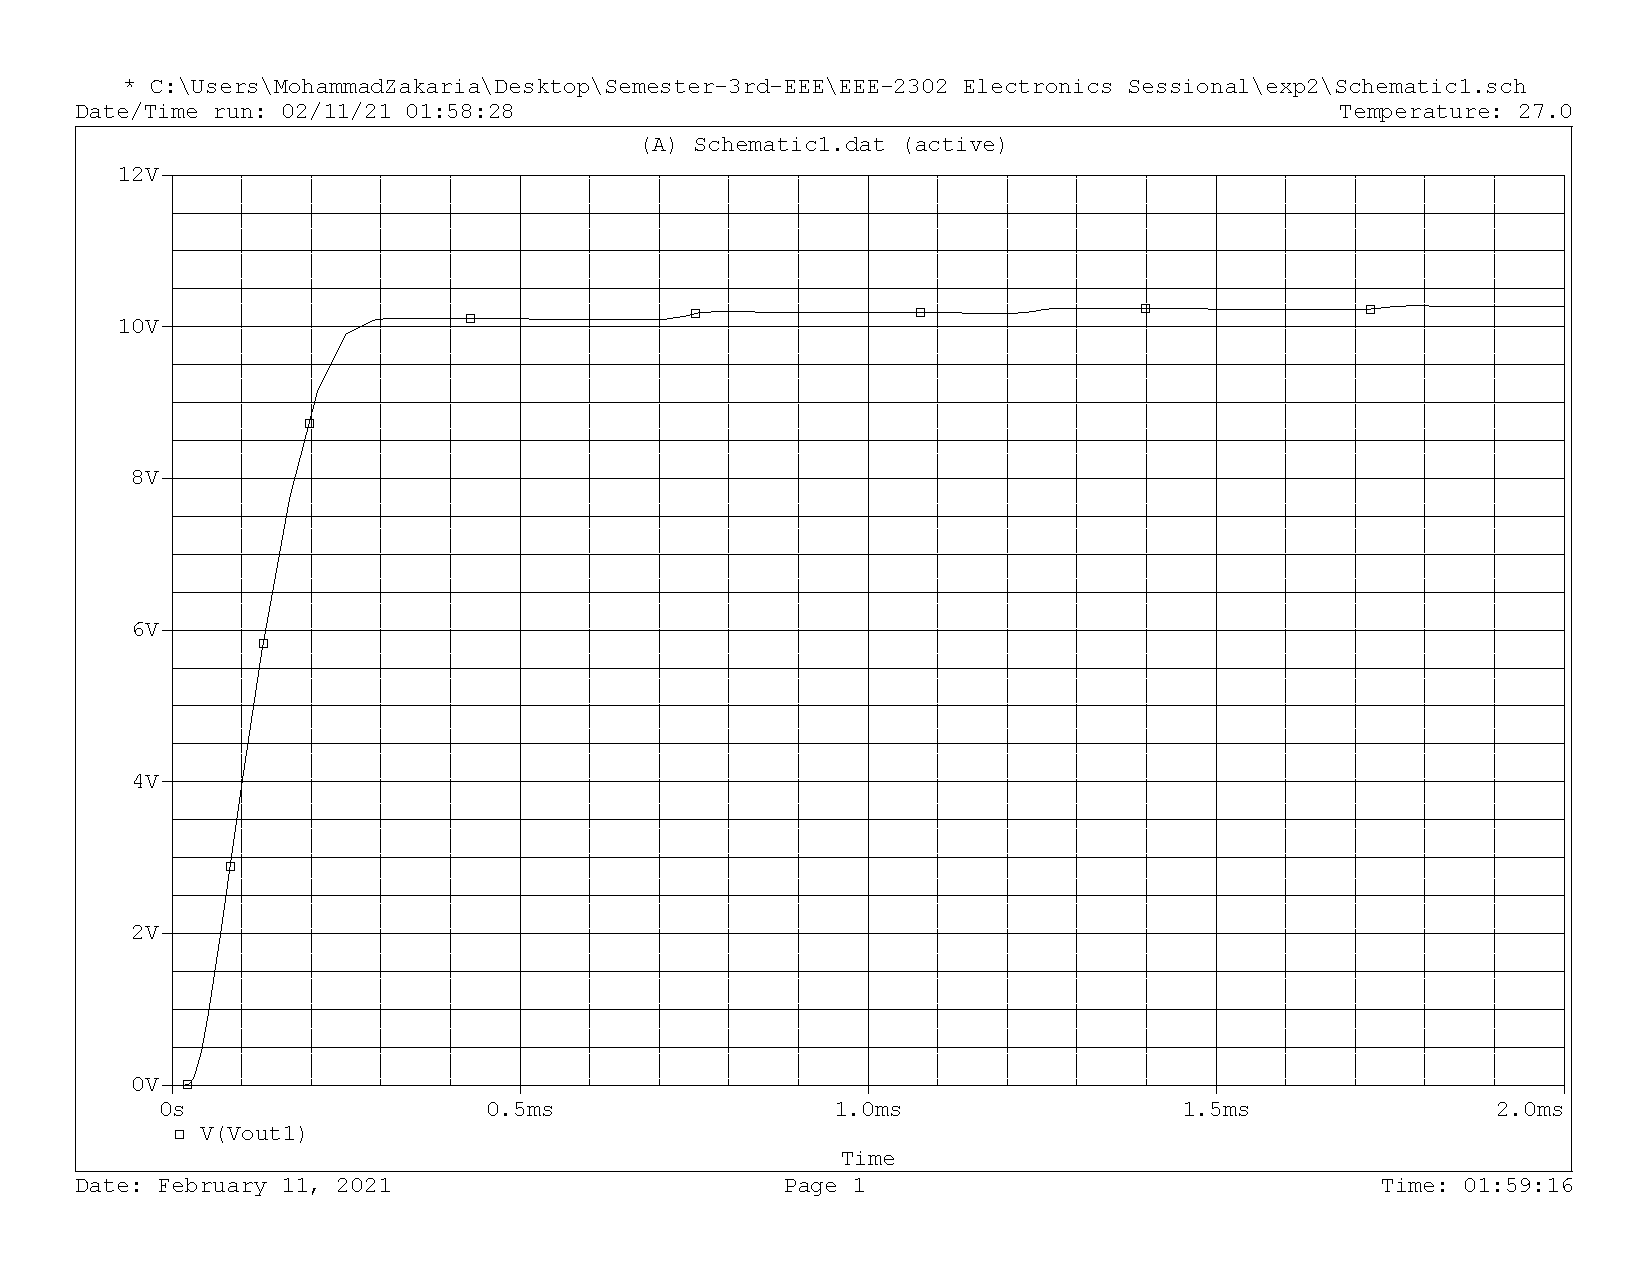
\includegraphics[width=0.7\linewidth]{Vout1-for-bride-fullwave-with-220ufd-capacitor.pdf}
		\caption{}
		\label{fig:vout1} Output voltage for full wave bridge rectifier when 220 \textmu F capacitor is connected.
	\end{figure}

	
\end{document}